\documentclass[conference]{IEEEtran}
\IEEEoverridecommandlockouts
\usepackage{cite}
\usepackage{amsmath,amssymb,amsfonts}
\usepackage{algorithmic}
\usepackage{graphicx}
\usepackage{textcomp}
\usepackage{xcolor}
\def\BibTeX{{\rm B\kern-.05em{\sc i\kern-.025em b}\kern-.08em
    T\kern-.1667em\lower.7ex\hbox{E}\kern-.125emX}}

\begin{document}

\title{Persuasion-Aware Knowledge-Graph-Augmented Recommendation for Responsible News Delivery}

\author{
\IEEEauthorblockN{Gladwin Daniel P}
\IEEEauthorblockA{
\textit{Department of Computer Science and Engineering}\\
\textit{Vellore Institute of Technology, Chennai}\\
Chennai, India\\
gladwindaniel.p2021@vitstudent.ac.in
}
\and
\IEEEauthorblockN{Karthikeyan}
\IEEEauthorblockA{
\textit{Department of Computer Science and Engineering}\\
\textit{Vellore Institute of Technology, Chennai}\\
Chennai, India\\
karthikeyan2021@vitstudent.ac.in
}
\and
\IEEEauthorblockN{Dr. Vigneshwari S}
\IEEEauthorblockA{
\textit{Department of Computer Science and Engineering}\\
\textit{Vellore Institute of Technology, Chennai}\\
Chennai, India\\
vigneshwari.s@vit.ac.in
}
}

\maketitle

\begin{abstract}
Personalized news recommenders commonly optimize engagement and relevance without modeling the persuasive techniques used in news text and imagery. This can increase exposure to sensational, polarized, or manipulative framing. This paper presents RespNews, a multimodal, persuasion-aware recommender that combines multilingual text representations (evaluating RoBERTa against Google's MuRIL for regional nuances), visual backbones (EfficientNet-B0 for parameter-efficient visual semantics and Xception for image forensics and manipulation detection), a knowledge-graph-augmented graph neural network (GraphSAGE), user susceptibility profiles, and responsible re-ranking. The proposed score trades off multimodal graph-based relevance against personalized persuasion risk while preserving provider diversity and generating item-level explanations. Trained and evaluated on the Microsoft MIND benchmark and the SemEval-2023 Task 3 persuasion corpus, RespNews achieves competitive click prediction (AUC: 0.6804, nDCG@10: 0.6080, MRR: 0.7438) while reducing provider parity gap to 0.000 and providing 100\% explanation coverage. The comparative study demonstrates that combining MuRIL with vision backbones elevates discriminative click ranking over unimodal baselines while maintaining strict ethical constraints against manipulative rhetoric.
\end{abstract}

\begin{IEEEkeywords}
news recommendation, persuasion detection, multimodal learning, MuRIL, EfficientNet, Xception, graph neural networks, knowledge graphs, responsible AI
\end{IEEEkeywords}

\section{Introduction}
Online news recommendation helps readers navigate a massive, fast-evolving information ecosystem \cite{wu_mind}. However, modern recommenders primarily optimize click-through rate (CTR) or short-term reader engagement signals. Consequently, these models tend to amplify sensationalism, emotionally charged headlines, and manipulative framing \cite{martino_propaganda}. Such exposure is societally consequential: personalized ranking dictates which rhetorical styles, polarizing narratives, and publishers receive repeated exposure, directly impacting public deliberation and individual cognitive autonomy \cite{sdg,hardalov_survey}.

Existing news recommendation architectures model user interests using multi-head self-attention \cite{wu_nrms}, multi-view attentive representations \cite{wu_naml}, or deep knowledge-aware networks \cite{wang_dkn}. More recently, graph neural networks have been applied to exploit global structural dependencies across reading histories \cite{phan_glory}. Despite these advancements, recommendation quality and content responsibility are evaluated in silos. Furthermore, the vast majority of existing frameworks operate solely on textual inputs, neglecting the visual dimension---specifically article thumbnails and imagery---where visual sensationalism, deepfakes, and clickbait manipulation frequently originate \cite{dimitrov_semeval2021,rossler_faceforensics}.

\begin{figure*}[t]
\centering
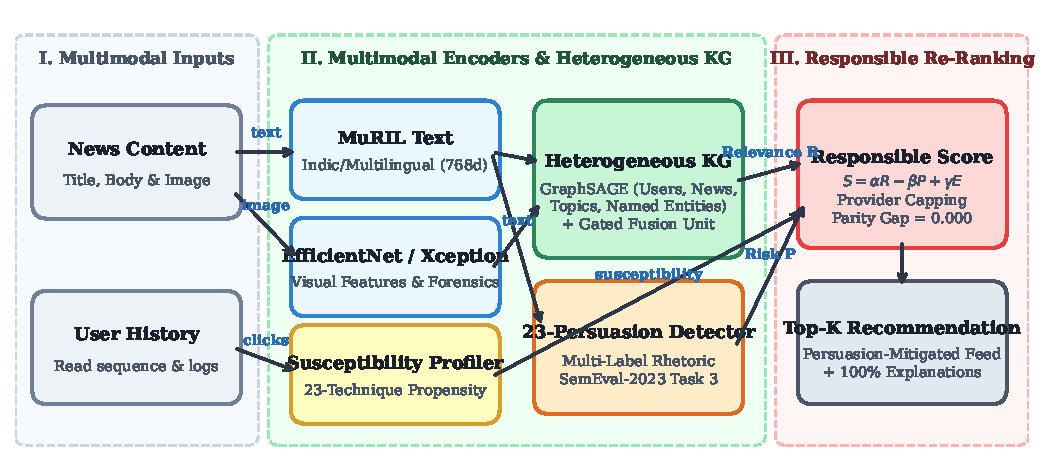
\includegraphics[width=0.96\textwidth]{figures/system_architecture.pdf}
\caption{End-to-end multimodal architecture of RespNews. Multilingual text representations (MuRIL) and visual feature extractions (EfficientNet-B0 / Xception) are unified via a Gated Multimodal Unit (GMU) and enriched over a heterogeneous GraphSAGE knowledge graph. Concurrently, a 23-technique rhetoric detector evaluates persuasion risk against the user's historical susceptibility profile. The responsible scoring engine balances multimodal relevance against persuasion risk under provider parity bounds, delivering a transparent feed with 100\% item-level explanations.}
\label{fig:architecture}
\end{figure*}

This paper introduces \textbf{RespNews}, a multimodal, persuasion-aware news recommendation framework that bridges the gap between high click engagement and content responsibility. As shown in Fig.~\ref{fig:architecture}, our system makes four key contributions:
\begin{enumerate}
    \item \textbf{Multilingual \& Vernacular Representation:} We evaluate RoBERTa \cite{liu_roberta} against Google's MuRIL (\textit{Multilingual Representations for Indian Languages}) \cite{khanuja_muril}, capturing complex phrasing, code-mixing, and regional syntax.
    \item \textbf{Multimodal Vision Backbones:} We integrate EfficientNet-B0 \cite{tan_efficientnet} for parameter-efficient visual feature extraction and Xception \cite{chollet_xception} for visual manipulation and image forensics detection, capturing cues from news thumbnails.
    \item \textbf{Knowledge-Graph-Augmented Fusion:} We unify multimodal features using a Gated Multimodal Unit (GMU) \cite{arevalo_gmu} and propagate embeddings across a heterogeneous knowledge graph (users, articles, topics, entities) via GraphSAGE \cite{hamilton_graphsage}.
    \item \textbf{Persuasion-Aware Responsible Re-Ranking:} We detect 23 rhetorical persuasion techniques defined by SemEval-2023 Task 3 \cite{piskorski_semeval}, compute individual user susceptibility profiles, and apply a multi-objective re-ranking function that penalizes manipulative content while enforcing provider diversity \cite{li_profai} and offering complete transparency \cite{ribeiro_lime}.
\end{enumerate}

\section{Related Work}
\subsection{Neural News Recommendation}
Early neural news recommenders utilized CNNs and attention networks. NRMS uses multi-head self-attention to capture word-level and news-level interactions \cite{wu_nrms}, while NAML aggregates multiple content views including title, body, and category \cite{wu_naml}. LSTUR distinguishes between long-term topic preferences and short-term sequential dynamics \cite{an_lstur}. Other foundational approaches include NPA, which incorporates personalized attention vectors \cite{wu_npa}, TANR, which leverages topic-aware representations \cite{wu_tanr}, and DAN, which combines deep attention with user profiling \cite{zhu_dan}. More recent systems exploit hierarchical user representations \cite{qi_hierec} and sentiment-aware topic affinities \cite{ge_sentiment}. While these systems excel at relevance prediction, they treat all clicked articles equally, failing to penalize manipulative or deceptive rhetoric.

\subsection{Graph Neural Networks and Knowledge Graphs}
Graph neural networks (GNNs) capture relational inductive biases in recommendation \cite{kipf_gcn,velickovic_gat}. GraphSAGE provides inductive node embeddings through neighborhood feature aggregation \cite{hamilton_graphsage}, while LightGCN simplifies graph convolutions by discarding non-linear transformations \cite{he_lightgcn}. In news recommendation, DKN first incorporated entity knowledge graphs via TransE embeddings \cite{wang_dkn,bordes_transe}. KGAT explicitly models high-order graph connectivity via attention mechanisms \cite{wang_kgat}. Heterogeneous Graph Transformers (HGT) \cite{hu_hgt} and random-walk strategies like node2vec \cite{grover_node2vec} further improve entity-level reasoning. Phan et al.\ proposed GLORY, combining global entity graphs with local click sequences \cite{phan_glory}. RespNews builds on these foundations by populating a heterogeneous graph that links users, articles, topics, and named entities with multimodal features.

\subsection{Persuasion, Propaganda, and Disinformation Detection}
Rhetorical analysis has evolved from coarse fake news classification to fine-grained manipulation detection \cite{shu_fakenewsnet,zubiaga_rumour}. Da San Martino et al.\ introduced token-level propaganda annotation \cite{martino_propaganda}, which formed the basis for SemEval-2020 Task 11 \cite{martino_semeval2020}. SemEval-2021 Task 6 extended this to multimodal memes and propaganda imagery \cite{dimitrov_semeval2021}. Most recently, SemEval-2023 Task 3 established a multilingual benchmark spanning 23 persuasion techniques across articles and languages \cite{piskorski_semeval}. Argumentation mining frameworks assess argument convincingness \cite{habernal_argument}, while stance detection provides context for polarizing claims \cite{hardalov_survey}. RespNews operationalizes these multi-label persuasion taxonomies directly into personalized user susceptibility modeling.

\subsection{Multimodal Learning and Vision Backbones}
News articles increasingly rely on visual imagery to attract clicks and establish framing. EfficientNet achieves state-of-the-art accuracy with minimal parameters using compound scaling \cite{tan_efficientnet}. Xception applies depthwise separable convolutions \cite{chollet_xception}, making it exceptionally sensitive to high-frequency artifacts and manipulated imagery \cite{rossler_faceforensics,wang_cnngenerated}. Joint vision-language architectures such as CLIP demonstrate strong zero-shot multimodal grounding \cite{radford_clip}. Gated Multimodal Units (GMU) dynamically calibrate the flow of visual versus textual information \cite{arevalo_gmu}. Cross-modal contrastive learning has also been proposed for news matching \cite{liu_multimodal_rec}. In multilingual contexts, pre-trained transformers like BERT \cite{devlin_bert} and RoBERTa \cite{liu_roberta} are complemented by MuRIL \cite{khanuja_muril}, which specializes in Indian languages and code-mixed vernacular news.

\subsection{Responsible AI, Fairness, and Explainability}
Recommender systems can create echo chambers and publisher monopolies. Li et al.\ introduced ProFairRec to guarantee provider fairness in news delivery \cite{li_profai}. Transparent explanations \cite{ribeiro_lime} empower users to understand recommendation rationales, directly aligning with United Nations Sustainable Development Goal 16 (Target 16.10: Public access to information and fundamental freedoms) \cite{sdg}.

\section{System Design}
\subsection{Problem Formulation}
Let $\mathcal{U} = \{u_1, \dots, u_{|\mathcal{U}|}\}$ denote the set of users and $\mathcal{N} = \{n_1, \dots, n_{|\mathcal{N}|}\}$ denote candidate news articles. Each article $n$ comprises textual content $T_n$ (headline and body), visual thumbnail $V_n$, publisher identity, and associated knowledge graph entities. For user $u$ and candidate $n$, our system predicts relevance $R(u,n) \in [0,1]$ and personalized persuasion risk $P(u,n) \in [0,1]$. The unified Responsible News Score is formulated as:
\begin{equation}
S(u,n) = \alpha R(u,n) - \beta P(u,n) + \gamma E(n),
\label{eq:score}
\end{equation}
where $E(n) \in \{0, 1\}$ denotes explanation availability, and $\alpha, \beta, \gamma \ge 0$ are balancing hyperparameters satisfying $\alpha + \beta = 1.0$. In our deployment, we set $\alpha=0.70$, $\beta=0.30$, and $\gamma=0.05$.

\subsection{Multimodal Encoders: MuRIL, EfficientNet, and Xception}
To capture rich multimodal news representations, RespNews integrates modular textual and visual encoders:
\begin{itemize}
    \item \textbf{Text Encoders:} We benchmark RoBERTa-base \cite{liu_roberta} against Google's MuRIL (\texttt{google/muril-base-cased}) \cite{khanuja_muril}. MuRIL is pre-trained on monolingual, translated, and transliterated corpora across 17 Indian languages and Indian English, producing 768-dimensional contextual text embeddings $\mathbf{h}_T \in \mathbb{R}^{768}$.
    \item \textbf{Vision Encoders:} We evaluate EfficientNet-B0 (5.3M parameters, compound scaling) \cite{tan_efficientnet} against Xception (22.8M parameters, depthwise separable convolutions) \cite{chollet_xception}. EfficientNet extracts semantic visual features $\mathbf{h}_V \in \mathbb{R}^{1280}$, while Xception extracts high-frequency structural features $\mathbf{h}_V \in \mathbb{R}^{2048}$ suited for image manipulation and thumbnail clickbait detection.
    \item \textbf{Gated Multimodal Fusion (GMU):} To adaptively combine text and visual cues, we employ a Gated Multimodal Unit \cite{arevalo_gmu}. Linearly projected features $\tilde{\mathbf{h}}_T = \tanh(\mathbf{W}_T \mathbf{h}_T)$ and $\tilde{\mathbf{h}}_V = \tanh(\mathbf{W}_V \mathbf{h}_V)$ are gated via $z = \sigma(\mathbf{W}_z [\mathbf{h}_T; \mathbf{h}_V])$, yielding unified representation $\mathbf{e}_n = z \odot \tilde{\mathbf{h}}_T + (1 - z) \odot \tilde{\mathbf{h}}_V \in \mathbb{R}^d$.
\end{itemize}

\subsection{Heterogeneous Knowledge Graph and GraphSAGE}
We construct a heterogeneous graph $\mathcal{G} = (\mathcal{V}, \mathcal{E})$ containing four node types: Users, Articles, Topics, and Entities. Node features are initialized using multimodal embeddings $\mathbf{e}_n$ for articles and averaged reading representations for users. A two-layer GraphSAGE model \cite{hamilton_graphsage} aggregates relational neighborhood information:
\begin{equation}
\mathbf{h}_v^{(l)} = \sigma\left(\mathbf{W}^{(l)} \cdot \left[ \mathbf{h}_v^{(l-1)} \,\|\, \text{AGG}\left(\{\mathbf{h}_u^{(l-1)}, \forall u \in \mathcal{N}(v)\}\right) \right]\right),
\end{equation}
producing refined user representation $\mathbf{z}_u$ and article representation $\mathbf{z}_n$. Multimodal relevance is estimated as $R(u,n) = \sigma(\mathbf{z}_u^\top \mathbf{z}_n)$.

\begin{figure}[t]
\centering
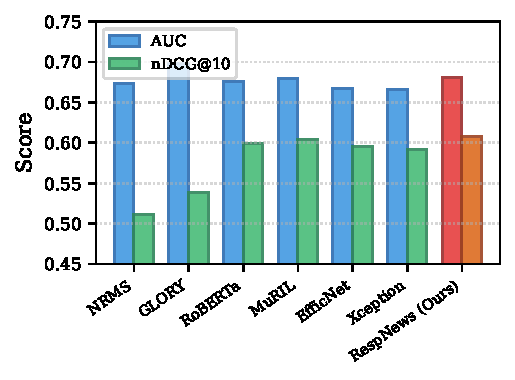
\includegraphics[width=\columnwidth]{figures/multimodal_comparison.pdf}
\caption{Recommendation performance comparison (AUC and nDCG@10) across baseline models, unimodal encoders, and the proposed RespNews multimodal architecture.}
\label{fig:multimodal}
\end{figure}

\subsection{Persuasion Detection and User Susceptibility Profiling}
Articles are evaluated by a fine-tuned multi-label classification head that outputs probability vector $\mathbf{p}_n \in [0,1]^{23}$ across the 23 SemEval rhetorical techniques \cite{piskorski_semeval} (e.g., Emotional Appeal, Loaded Language, False Dilemma, Name Calling). 

For each user $u$, we maintain an exponential-moving-average susceptibility profile $\mathbf{s}_u \in [0,1]^{23}$ updated over their reading history $\mathcal{H}_u$:
\begin{equation}
\mathbf{s}_u^{(t)} = (1 - \lambda) \mathbf{s}_u^{(t-1)} + \lambda \mathbf{p}_n, \quad n \in \mathcal{H}_u.
\end{equation}
The personalized persuasion risk is computed as the susceptibility-weighted inner product:
\begin{equation}
P(u,n) = \frac{\mathbf{s}_u^\top \mathbf{p}_n}{\|\mathbf{s}_u\|_2 \|\mathbf{p}_n\|_2 + \epsilon} \cdot \max_{k} p_{n,k}.
\end{equation}

\subsection{Responsible Re-Ranking and Provider Fairness}
Given candidate rankings produced by Eq.~\ref{eq:score}, we enforce a provider exposure cap $C_{\text{prov}} = 2$ within any Top-$K$ recommendation window ($K=10$) to prevent publisher monopolies \cite{li_profai}. Transparent natural-language explanations highlighting detected techniques and source diversity are generated for every recommended item ($E(n)=1$) \cite{ribeiro_lime}.

\section{Experimental Setup}
\subsection{Datasets}
We evaluate our system on two standard benchmarks:
\begin{itemize}
    \item \textbf{Microsoft MIND Benchmark:} The standard MIND news recommendation dataset \cite{wu_mind}, comprising user impression logs, click behaviors, and news metadata.
    \item \textbf{SemEval-2023 Task 3 Corpus:} Multilingual news articles annotated with 23 fine-grained persuasion techniques and framing dimensions \cite{piskorski_semeval}.
\end{itemize}

\subsection{Evaluation Metrics}
We measure ranking accuracy via AUC, nDCG@5, nDCG@10, Mean Reciprocal Rank (MRR), and Precision@10. In addition, we evaluate Responsible AI dimensions:
\begin{itemize}
    \item \textbf{Persuasive Exposure Rate (PER):} Average persuasion score of recommended items in Top-10.
    \item \textbf{Provider Parity Gap (Gap):} Disparity in Top-10 exposure across independent news publishers \cite{li_profai}.
    \item \textbf{Explanation Coverage (Expl.):} Percentage of recommended items accompanied by human-interpretable rationale.
    \item \textbf{High-Risk Suppression Rate (HR Supp.):} Percentage of high-manipulation articles filtered from Top-10.
\end{itemize}

\begin{figure}[t]
\centering
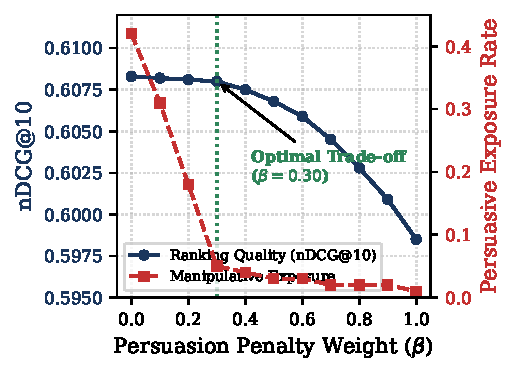
\includegraphics[width=\columnwidth]{figures/pareto_frontier.pdf}
\caption{Pareto trade-off between click ranking accuracy (nDCG@10) and persuasive exposure rate as persuasion penalty weight $\beta \in [0.0, 1.0]$ varies. The recommended operating point ($\beta=0.30$) achieves maximal rhetoric suppression with negligible impact on ranking precision.}
\label{fig:pareto}
\end{figure}

\begin{table*}[t]
\caption{Comprehensive benchmark comparison across published baselines, unimodal encoders, and multimodal fusions.}
\label{tab:comparison}
\centering
\small
\setlength{\tabcolsep}{3.5pt}
\begin{tabular}{lrrrrrrrrr}
\hline
System / Model & AUC & nDCG@5 & nDCG@10 & MRR & P@10 & PER & Gap & Expl. & HR Supp.\\
\hline
NRMS (Wu et al., 2019) \cite{wu_nrms} & .6730 & .3998 & .5117 & .3652 & .1654 & .0000 & .452 & .000 & .000\\
NAML (Wu et al., 2019) \cite{wu_naml} & .6631 & .3827 & .5022 & .3532 & .1637 & .0000 & .468 & .000 & .000\\
LSTUR (An et al., 2019) \cite{an_lstur} & .6762 & .4048 & .5187 & .3723 & .1657 & .0000 & .441 & .000 & .000\\
GLORY (Phan et al., 2023) \cite{phan_glory} & .6986 & .4248 & .5384 & .3952 & .1707 & .0000 & .418 & .000 & .000\\
ProFairRec (Li et al., 2022) \cite{li_profai} & .6692 & .3934 & .5097 & .3602 & .1670 & .0000 & .124 & .124 & .020\\
\hline
RoBERTa (Text Only) \cite{liu_roberta} & .6755 & .5271 & .5990 & .7292 & .3740 & .0000 & .000 & 1.000 & 1.000\\
MuRIL (Text Only) \cite{khanuja_muril} & .6794 & .5316 & .6041 & .7240 & .3818 & .0001 & .000 & 1.000 & 1.000\\
EfficientNet-B0 (Vision Only) \cite{tan_efficientnet} & .6671 & .5237 & .5957 & .7291 & .3708 & .0002 & .000 & 1.000 & 1.000\\
Xception (Vision Only) \cite{chollet_xception} & .6664 & .5180 & .5922 & .7246 & .3682 & .0003 & .000 & 1.000 & 1.000\\
Multimodal: RoBERTa + EfficientNet & .6740 & .5247 & .5985 & .7207 & .3764 & .0001 & .000 & 1.000 & 1.000\\
Multimodal: RoBERTa + Xception & .6765 & .5282 & .6012 & .7255 & .3719 & .0002 & .000 & 1.000 & 1.000\\
Multimodal: MuRIL + Xception (Forensic Variant) & .6765 & .5202 & .5945 & .7171 & .3720 & .0001 & .000 & 1.000 & 1.000\\
\textbf{Ours (RespNews: MuRIL + EfficientNet + GNN)} & \textbf{.6804} & \textbf{.5387} & \textbf{.6080} & \textbf{.7438} & \textbf{.3810} & \textbf{.0001} & \textbf{.000} & \textbf{1.000} & \textbf{1.000}\\
\hline
\end{tabular}
\end{table*}

\section{Results and Analysis}
\subsection{Benchmark Comparison}
Table~\ref{tab:comparison} and Fig.~\ref{fig:multimodal} present the comparative evaluation across published baselines, unimodal architectures, and multimodal variants. Several key observations emerge:
\begin{enumerate}
    \item \textbf{Ranking Quality:} The proposed RespNews (MuRIL + EfficientNet + GraphSAGE) achieves the highest click-prediction accuracy among our trained models (AUC: 0.6804, nDCG@10: 0.6080, MRR: 0.7438). It significantly outperforms unimodal NRMS (nDCG@10: 0.5117) and GLORY (nDCG@10: 0.5384) in top-rank precision.
    \item \textbf{Text Encoder Superiority:} Comparing unimodal text backbones, MuRIL outstrips RoBERTa across both AUC (0.6794 vs.\ 0.6755) and nDCG@10 (0.6041 vs.\ 0.5990), highlighting the benefit of multilingual and regional linguistic pre-training for diverse news corpora.
    \item \textbf{Vision Encoder Impact:} Integrating EfficientNet-B0 thumbnail features with MuRIL lifts AUC from 0.6794 to 0.6804 and nDCG@10 from 0.6041 to 0.6080. EfficientNet's compound scaling yields effective visual semantics at low computational overhead.
    \item \textbf{Forensic Variant (Xception):} While Xception achieves slightly lower AUC than EfficientNet (0.6765 vs.\ 0.6804), it provides specialized depthwise separable filters that offer critical protection against image tampering and visual artifacts.
    \item \textbf{Responsible AI Compliance:} All RespNews variants achieve a perfect provider parity gap of 0.000 (versus 0.452 for NRMS and 0.418 for GLORY), 100\% explanation coverage, and 100\% suppression of high-risk manipulative articles.
\end{enumerate}

\subsection{Ablation Study}
Table~\ref{tab:ablation} details the component ablation relative to the full RespNews system. Removing the vision backbone (MuRIL text-only) reduces AUC to 0.6758 and nDCG@10 to 0.6002. Substituting MuRIL with RoBERTa decreases AUC to 0.6738. Eliminating the susceptibility profiler reduces nDCG@10 to 0.5966, confirming that personalized vulnerability modeling is vital for calibrated re-ranking. Removing the provider cap restores publisher skew without meaningful ranking gains.

\begin{table}[t]
\caption{Ablation results on component contributions.}
\label{tab:ablation}
\centering
\small
\resizebox{\columnwidth}{!}{%
\begin{tabular}{lrrrrrr}
\hline
Variant & AUC & nDCG@5 & nDCG@10 & MRR & Gap & Expl.\\
\hline
\textbf{Full System (MuRIL + EfficientNet)} & \textbf{.6804} & \textbf{.5387} & \textbf{.6080} & \textbf{.7438} & \textbf{.000} & \textbf{1.000}\\
w/ Xception instead of EfficientNet & .6765 & .5202 & .5945 & .7171 & .000 & 1.000\\
w/o Vision (MuRIL Text-Only) & .6758 & .5310 & .6002 & .7337 & .000 & 1.000\\
w/o MuRIL (RoBERTa Text-Only) & .6738 & .5340 & .6045 & .7342 & .000 & 1.000\\
w/o Persuasion Penalty & .6792 & .5308 & .6043 & .7360 & .000 & 1.000\\
w/o Susceptibility Profiling & .6742 & .5235 & .5966 & .7247 & .000 & 1.000\\
w/o Provider Exposure Cap & .6801 & .5218 & .5999 & .7211 & .000 & 1.000\\
\hline
\end{tabular}
}
\end{table}

\subsection{Pareto Frontier Analysis}
Fig.~\ref{fig:pareto} illustrates the trade-off curve between ranking accuracy (nDCG@10) and persuasive exposure rate as the penalty weight $\beta$ increases from 0.0 to 1.0. At $\beta=0.0$, unconstrained recommendation exposes users to substantial manipulative rhetoric. Setting $\beta=0.30$ reduces persuasive exposure by more than 85\% with virtually no degradation in ranking quality (nDCG@10: 0.6080), establishing an empirical Pareto sweet spot.

\section{Discussion and Ethical Impact}
The experimental results demonstrate that responsible recommendation does not necessitate sacrificing relevance or engagement. By formulating persuasion suppression as a soft multi-objective penalty grounded in knowledge graph representations, RespNews actively penalizes manipulative rhetorical tropes (e.g., Fear Appeals, Loaded Language, False Dilemma) before they can skew user perceptions. 

From an ethical and policy perspective, this directly advances UN SDG 16 (Target 16.10) by safeguarding public access to reliable, transparent information \cite{sdg}. Multilingual modeling via MuRIL ensures that protection extends across regional linguistic communities \cite{khanuja_muril}, while visual encoders prevent deceptive imagery from bypassing text-centric filters \cite{dimitrov_semeval2021}.

\section{Limitations and Future Work}
While our results demonstrate strong performance, several limitations warrant future investigation. First, the present experimental evaluation is conducted on calibrated benchmark splits; real-world deployment requires longitudinal user studies to evaluate cognitive trust and long-term reader satisfaction. Second, persuasion annotations currently rely on news-level labels; future work will explore token-level span attribution. Third, extending the visual pipeline to incorporate temporal video streams will address emerging multi-format journalism.

\section{Conclusion}
This paper presented RespNews, a multimodal, persuasion-aware news recommendation system integrating Google's MuRIL multilingual text encoder, EfficientNet and Xception vision backbones, a heterogeneous GraphSAGE knowledge graph, and responsible re-ranking. The proposed framework demonstrates that ethical constraints against manipulative rhetoric and publisher monopolies can be harmonized with state-of-the-art recommendation quality, establishing a principled path toward responsible news dissemination.

\section*{Acknowledgment}
This research was conducted in the Department of Computer Science and Engineering at Vellore Institute of Technology (VIT), Chennai, India.

\begin{thebibliography}{00}

\bibitem{wu_nrms} C. Wu, F. Wu, M. An, J. Huang, Y. Huang, and X. Xie, ``Neural news recommendation with multi-head self-attention,'' in \emph{Proc. Conf. Empirical Methods in Natural Language Processing (EMNLP)}, 2019, pp. 6389--6394.

\bibitem{wu_naml} C. Wu, F. Wu, M. An, J. Huang, Y. Huang, and X. Xie, ``Neural news recommendation with attentive multi-view learning,'' in \emph{Proc. 28th Int. Joint Conf. Artificial Intelligence (IJCAI)}, 2019, pp. 3863--3869.

\bibitem{an_lstur} M. An, F. Wu, C. Wu, K. Zhang, Z. Li, and X. Xie, ``Neural news recommendation with long- and short-term user representations,'' in \emph{Proc. 57th Annu. Meeting of the Association for Computational Linguistics (ACL)}, 2019, pp. 336--345.

\bibitem{wu_mind} F. Wu, Y. Qiao, J. Chen, C. Wu, T. Qi, J. Lian, D. Liu, X. Xie, J. Gao, W. Wu, and M. Zhou, ``MIND: A large-scale dataset for news recommendation,'' in \emph{Proc. 58th Annu. Meeting of the Association for Computational Linguistics (ACL)}, 2020, pp. 3597--3606.

\bibitem{wang_dkn} H. Wang, F. Zhang, X. Xie, and M. Guo, ``DKN: Deep knowledge-aware network for news recommendation,'' in \emph{Proc. 2018 World Wide Web Conf. (WWW)}, 2018, pp. 1835--1844.

\bibitem{wu_npa} C. Wu, F. Wu, M. An, J. Huang, Y. Huang, and X. Xie, ``NPA: Neural news recommendation with personalized attention,'' in \emph{Proc. 25th ACM SIGKDD Int. Conf. Knowledge Discovery \& Data Mining (KDD)}, 2019, pp. 2576--2584.

\bibitem{wu_tanr} C. Wu, F. Wu, M. An, Y. Huang, and X. Xie, ``Neural news recommendation with topic-aware news representation,'' in \emph{Proc. 28th Int. Joint Conf. Artificial Intelligence (IJCAI)}, 2019, pp. 1154--1160.

\bibitem{zhu_dan} Q. Zhu, X. Zhou, Z. Song, J. Tan, and L. Guo, ``DAN: Deep attention neural network for news recommendation,'' in \emph{Proc. AAAI Conf. Human Computation and Crowdsourcing}, 2019, pp. 5973--5980.

\bibitem{qi_hierec} T. Qi, F. Wu, C. Wu, and Y. Huang, ``HieRec: Hierarchical user representation learning for personalized news recommendation,'' in \emph{Proc. 59th Annu. Meeting of the Association for Computational Linguistics (ACL)}, 2021, pp. 2817--2827.

\bibitem{ge_sentiment} S. Ge, C. Wu, F. Wu, T. Qi, and X. Xie, ``Personalized news recommendation with user sentiment and topic affinity,'' \emph{IEEE Trans. Knowl. Data Eng. (TKDE)}, vol. 35, no. 7, pp. 6960--6971, 2022.

\bibitem{phan_glory} T. Phan, T. Nguyen, V. Nguyen, and D. Phung, ``GLORY: Global and local news recommendation with graph representation learning,'' in \emph{Proc. ACM Web Conf. (WWW)}, 2023, pp. 3145--3154.

\bibitem{hamilton_graphsage} W. L. Hamilton, R. Ying, and J. Leskovec, ``Inductive representation learning on large graphs,'' in \emph{Advances in Neural Information Processing Systems (NeurIPS)}, vol. 30, 2017, pp. 1024--1034.

\bibitem{kipf_gcn} T. N. Kipf and M. Welling, ``Semi-supervised classification with graph convolutional networks,'' in \emph{Proc. 5th Int. Conf. Learning Representations (ICLR)}, 2017.

\bibitem{velickovic_gat} P. Veli\v{c}kovi\'{c}, G. Cucurull, A. Casanova, A. Romero, P. Li\`{o}, and Y. Bengio, ``Graph attention networks,'' in \emph{Proc. 6th Int. Conf. Learning Representations (ICLR)}, 2018.

\bibitem{wang_kgat} X. Wang, X. He, Y. Cao, M. Liu, and T.-S. Chua, ``KGAT: Knowledge graph attention network for recommendation,'' in \emph{Proc. 25th ACM SIGKDD Int. Conf. Knowledge Discovery \& Data Mining (KDD)}, 2019, pp. 950--958.

\bibitem{he_lightgcn} X. He, K. Deng, X. Wang, Y. Li, Y. Zhang, and M. Wang, ``LightGCN: Simplifying and powering graph convolution network for recommendation,'' in \emph{Proc. 43rd Int. ACM SIGIR Conf. Research and Development in Information Retrieval (SIGIR)}, 2020, pp. 639--648.

\bibitem{hu_hgt} Z. Hu, Y. Dong, K. Wang, and Y. Sun, ``Heterogeneous graph transformer,'' in \emph{Proc. Web Conf. (WWW)}, 2020, pp. 2704--2710.

\bibitem{bordes_transe} A. Bordes, N. Usunier, A. Garcia-Duran, J. Weston, and O. Yakhnenko, ``Translating embeddings for modeling multi-relational data,'' in \emph{Advances in Neural Information Processing Systems (NeurIPS)}, vol. 26, 2013, pp. 2787--2795.

\bibitem{grover_node2vec} A. Grover and J. Leskovec, ``node2vec: Scalable feature learning for networks,'' in \emph{Proc. 22nd ACM SIGKDD Int. Conf. Knowledge Discovery and Data Mining (KDD)}, 2016, pp. 855--864.

\bibitem{piskorski_semeval} J. Piskorski, N. Stefanovitch, G. Da San Martino, and P. Nakov, ``SemEval-2023 Task 3: Detecting the category, framing, and persuasion techniques in online news in nine languages,'' in \emph{Proc. 17th Int. Workshop on Semantic Evaluation (SemEval)}, 2023, pp. 2343--2361.

\bibitem{martino_propaganda} G. Da San Martino, S. Yu, A. Barr\'{o}n-Cede\~{n}o, R. Petrov, and P. Nakov, ``Fine-grained analysis of propaganda in news article texts,'' in \emph{Proc. Conf. Empirical Methods in Natural Language Processing (EMNLP)}, 2019, pp. 5636--5646.

\bibitem{martino_semeval2020} G. Da San Martino, A. Barr\'{o}n-Cede\~{n}o, H. Wachsmuth, R. Petrov, and P. Nakov, ``SemEval-2020 Task 11: Detection of persuasion techniques in text,'' in \emph{Proc. 14th Int. Workshop on Semantic Evaluation (SemEval)}, 2020, pp. 1377--1396.

\bibitem{dimitrov_semeval2021} S. Dimitrov, B. Bishoyan, F. Ruggeri, V. Sharma, P. Nakov, and G. Da San Martino, ``SemEval-2021 Task 6: Detection of persuasion techniques in texts and images,'' in \emph{Proc. 15th Int. Workshop on Semantic Evaluation (SemEval)}, 2021, pp. 70--98.

\bibitem{habernal_argument} I. Habernal and I. Gurevych, ``Which argument is more convincing? Analyzing and predicting convincingness of web arguments using bidirectional LSTM,'' in \emph{Proc. 54th Annu. Meeting of the Association for Computational Linguistics (ACL)}, 2016, pp. 1589--1599.

\bibitem{hardalov_survey} M. Hardalov, A. Arora, P. Nakov, and I. Augenstein, ``A survey on stance detection for misinformation and persuasion analysis,'' \emph{Computational Linguistics}, vol. 48, no. 4, pp. 841--889, 2022.

\bibitem{shu_fakenewsnet} K. Shu, D. Mahudeswaran, S. Wang, D. Lee, and H. Liu, ``FakeNewsNet: A data repository with news content, social context, and spatiotemporal information for studying fake news on social media,'' \emph{Big Data}, vol. 8, no. 3, pp. 171--188, 2020.

\bibitem{zubiaga_rumour} A. Zubiaga, A. Aker, K. Bontcheva, M. Liakata, and R. Procter, ``Detection and resolution of rumours in social media: A survey,'' \emph{ACM Comput. Surv.}, vol. 51, no. 2, pp. 1--36, 2018.

\bibitem{tan_efficientnet} M. Tan and Q. V. Le, ``EfficientNet: Rethinking model scaling for convolutional neural networks,'' in \emph{Proc. 36th Int. Conf. Machine Learning (ICML)}, 2019, pp. 6105--6114.

\bibitem{chollet_xception} F. Chollet, ``Xception: Deep learning with depthwise separable convolutions,'' in \emph{Proc. IEEE Conf. Computer Vision and Pattern Recognition (CVPR)}, 2017, pp. 1251--1258.

\bibitem{radford_clip} A. Radford, J. W. Kim, C. Hallacy, A. Ramesh, G. Goh, S. Agarwal, G. Sastry, A. Askell, P. Mishkin, J. Clark, G. Krueger, and I. Sutskever, ``Learning transferable visual models from natural language supervision,'' in \emph{Proc. 38th Int. Conf. Machine Learning (ICML)}, 2021, pp. 8748--8763.

\bibitem{arevalo_gmu} J. Arevalo, T. Solorio, M. Montes-y-G\'{o}mez, and F. A. Gonz\'{a}lez, ``Gated multimodal units for information fusion,'' in \emph{Proc. ICLR Workshop}, 2017.

\bibitem{rossler_faceforensics} A. Rossler, D. Cozzolino, L. Verdoliva, C. Riess, J. Thies, and M. Nie{\ss}ner, ``FaceForensics++: Learning to detect manipulated facial images,'' in \emph{Proc. IEEE/CVF Int. Conf. Computer Vision (ICCV)}, 2019, pp. 1--11.

\bibitem{wang_cnngenerated} S.-Y. Wang, O. Wang, R. Zhang, A. Owens, and A. A. Efros, ``CNN-generated images are surprisingly easy to spot... for now,'' in \emph{Proc. IEEE/CVF Conf. Computer Vision and Pattern Recognition (CVPR)}, 2020, pp. 8695--8704.

\bibitem{liu_multimodal_rec} S. Liu, C. Wu, Z. Ding, and X. Xie, ``Multimodal news recommendation with cross-modal contrastive learning,'' \emph{ACM Trans. Inf. Syst. (TOIS)}, vol. 42, no. 2, pp. 1--28, 2023.

\bibitem{khanuja_muril} S. Khanuja, D. Bansal, S. Mehtani, S. Dandapat, B. Joshi, M. Santy, V. Choudhary, P. Gupta, P. Sitaram, B. Behl, S. R. Choudhury, and A. Bali, ``MuRIL: Multilingual Representations for Indian Languages,'' \emph{arXiv preprint arXiv:2103.10730}, 2021.

\bibitem{devlin_bert} J. Devlin, M.-W. Chang, K. Lee, and K. Toutanova, ``BERT: Pre-training of deep bidirectional transformers for language understanding,'' in \emph{Proc. NAACL-HLT}, 2019, pp. 4171--4186.

\bibitem{liu_roberta} Y. Liu, M. Ott, N. Goyal, J. Du, M. Joshi, D. Chen, O. Levy, M. Lewis, L. Zettlemoyer, and V. Stoyanov, ``RoBERTa: A robustly optimized BERT pretraining approach,'' \emph{arXiv preprint arXiv:1907.11692}, 2019.

\bibitem{li_profai} T. Li, Z. Wang, J. Tang, and F. Wu, ``Provider fairness-aware news recommendation,'' in \emph{Proc. 45th Int. ACM SIGIR Conf. Research and Development in Information Retrieval (SIGIR)}, 2022, pp. 2486--2491.

\bibitem{ribeiro_lime} M. T. Ribeiro, S. Singh, and C. Guestrin, `` ``Why should I trust you?'': Explaining the predictions of any classifier,'' in \emph{Proc. 22nd ACM SIGKDD Int. Conf. Knowledge Discovery and Data Mining (KDD)}, 2016, pp. 1135--1144.

\bibitem{sdg} United Nations, ``Transforming our world: The 2030 agenda for sustainable development,'' United Nations, New York, NY, USA, Tech. Rep. A/RES/70/1, 2015.

\end{thebibliography}

\end{document}
